%%%%%%%%%%%%%%%%%%%%%%%%%%%%%%%%%%%%%%%%%
% Beamer Presentation
% LaTeX Template
% Version 1.0 (10/11/12)
%
% This template has been downloaded from:
% http://www.LaTeXTemplates.com
%
% License:
% CC BY-NC-SA 3.0 (http://creativecommons.org/licenses/by-nc-sa/3.0/)
%
%%%%%%%%%%%%%%%%%%%%%%%%%%%%%%%%%%%%%%%%%

%----------------------------------------------------------------------------------------
%	PACKAGES AND THEMES
%----------------------------------------------------------------------------------------

\documentclass{beamer}

\mode<presentation> {

% The Beamer class comes with a number of default slide themes
% which change the colors and layouts of slides. Below this is a list
% of all the themes, uncomment each in turn to see what they look like.

%\usetheme{default}
%\usetheme{AnnArbor}
%\usetheme{Antibes}
%\usetheme{Bergen}
%\usetheme{Berkeley}
%\usetheme{Berlin}
%\usetheme{Boadilla}
\usetheme{CambridgeUS}
%\usetheme{Copenhagen}
%\usetheme{Darmstadt}
%\usetheme{Dresden}
%\usetheme{Frankfurt}
%\usetheme{Goettingen}
%\usetheme{Hannover}
%\usetheme{Ilmenau}
%\usetheme{JuanLesPins}
%\usetheme{Luebeck}
%\usetheme{Madrid}
%\usetheme{Malmoe}
%\usetheme{Marburg}
%\usetheme{Montpellier}
%\usetheme{PaloAlto}
%\usetheme{Pittsburgh}
%\usetheme{Rochester}
%\usetheme{Singapore}
%\usetheme{Szeged}
%\usetheme{Warsaw}

% As well as themes, the Beamer class has a number of color themes
% for any slide theme. Uncomment each of these in turn to see how it
% changes the colors of your current slide theme.

%\usecolortheme{albatross}
%\usecolortheme{beaver}
%\usecolortheme{beetle}
%\usecolortheme{crane}
%\usecolortheme{dolphin}
%\usecolortheme{dove}
%\usecolortheme{fly}
%\usecolortheme{lily}
%\usecolortheme{orchid}
%\usecolortheme{rose}
%\usecolortheme{seagull}
%\usecolortheme{seahorse}
%\usecolortheme{whale}
%\usecolortheme{wolverine}

%\setbeamertemplate{footline} % To remove the footer line in all slides uncomment this line
%\setbeamertemplate{footline}[page number] % To replace the footer line in all slides with a simple slide count uncomment this line

%\setbeamertemplate{navigation symbols}{} % To remove the navigation symbols from the bottom of all slides uncomment this line
}

\usepackage{graphicx} % Allows including images
\usepackage{booktabs} % Allows the use of \toprule, \midrule and \bottomrule in tables

%----------------------------------------------------------------------------------------
%	TITLE PAGE
%----------------------------------------------------------------------------------------

\title[AlmaNotes]{Elaborato ASW: AlmaNotes} % The short title appears at the bottom of every slide, the full title is only on the title page

\author{Bombardi, Mascellaro, Ragazzi} % Your name
\institute[UNIBO] % Your institution as it will appear on the bottom of every slide, may be shorthand to save space
{
\medskip
\textbf{Corso di Laurea Magistrale in Ingegneria e Scienze Informatiche} \\ % Your institution for the title page
\medskip
\medskip
\textbf{Applicazioni e Servizi Web - Elaborato} \\ % Your institution for the title page
\medskip
}
\date{12/11/2019} % Date, can be changed to a custom date

\begin{document}

\begin{frame}
\titlepage % Print the title page as the first slide
\end{frame}

\begin{frame}
\frametitle{Overview} % Table of contents slide, comment this block out to remove it
\tableofcontents % Throughout your presentation, if you choose to use \section{} and \subsection{} commands, these will automatically be printed on this slide as an overview of your presentation
\end{frame}

%----------------------------------------------------------------------------------------
%	PRESENTATION SLIDES
%----------------------------------------------------------------------------------------

\section{Design}

%------------------------------------------------
\subsection{Goal \& Target Group}

\begin{frame}
\frametitle{Goal \& Target Group}
\begin{block}{Goal}
L'obiettivo dell'elaborato è realizzare un'applicazione web per la condivisione di materiale didattico (appunti e libri di testo) tra studenti all’interno del Nuovo Campus Universitario di Cesena.
\end{block}
\begin{block}{Target Group}
Il target group dell'applicazione, ossia il gruppo di utenti a cui essa è rivolta, è costituito dagli studenti iscritti ad un corso di laurea ospitato dal Nuovo Campus Universitario di Cesena. Si tratta di un target specifico che ci consente di affermare, ad esempio, che gli utenti non saranno completamente nuovi all'utilizzo di app di questo tipo (uno studente potrebbe non utilizzare applicazioni web o mobile ma, essendo un iscritto UNIBO, talvolta deve accedere a piattaforme come StudentiOnline).
\end{block}
\end{frame}
%------------------------------------------------
\subsection{Personas \& Scenarios}

\begin{frame}
\frametitle{Personas \& Scenarios: Camilla}
\begin{figure}

\includegraphics[width=0.15\linewidth]{images/user_f.png}
\end{figure}
\begin{block}{}
Camilla ha 20 anni ed è una studentessa che, sin dai tempi del liceo, è affascinata dal mondo della scienza e ha il sogno di lavorare nel campo delle protesi artificiali. Nonostante le difficoltà economiche della sua famiglia, Camilla ha vinto una borsa di studio che le ha consentito di trasferirsi a Cesena e iscriversi alla LT in Ingegneria Biomedica.
\end{block}
\begin{block}{Scenario}
Camilla utilizza l'applicazione per cercare e richiedere in prestito libri utili al suo percorso di studi e che non può permettersi di comprare. Inoltre, tramite l'app Camilla mette a disposizione i suoi appunti.
\end{block}
\end{frame}
\begin{frame}
\frametitle{Personas \& Scenarios: Giulio}
\begin{figure}

\includegraphics[width=0.17\linewidth]{images/user.png}
\end{figure}
\begin{block}{}
Giulio ha 23 anni ed è uno studente lavoratore iscritto al primo anno della LM in Ingegneria e Scienze Informatiche. A causa dei suoi impegni lavorativi, Giulio può frequentare le lezioni solo una volta a settimana.
\end{block}
\begin{block}{Scenario}
Grazie all'applicazione Giulio recupera appunti relativi ai corsi che non riesce a seguire e cerca di rimanere al passo con le lezioni. Per sdebitarsi carica nella piattaforma i suoi vecchi libri, quelli utilizzati durante la LT.
\end{block}
\end{frame}
\begin{frame}
\frametitle{Personas \& Scenarios: Nicola}
\begin{figure}

\includegraphics[width=0.18\linewidth]{images/user_s.png}
\end{figure}
\begin{block}{}
Nicola ha 21 anni ed è iscritto al terzo anno della LT in Ingegneria Elettronica. Grazie alla sua passione per la materia e agli ottimi risultati raggiunti, è ormai prossimo alla laurea e può essere definito uno “studente modello". Durante la sua esperienze universitaria Nicola ha accumulato appunti e libri relativi a diverse materie, che ora non utilizza più.
\end{block}
\begin{block}{Scenario}
Nicola usa l'applicazione per condividere i suoi appunti e i suoi libri e, con i punti guadagnati, può sempre riempire gratuitamente la sua borraccia.
\end{block}
\end{frame}
%------------------------------------------------
\subsection{Storyboard}

\begin{frame}
\frametitle{Storyboard: Prendere in prestito un documento (1)}
\begin{figure}
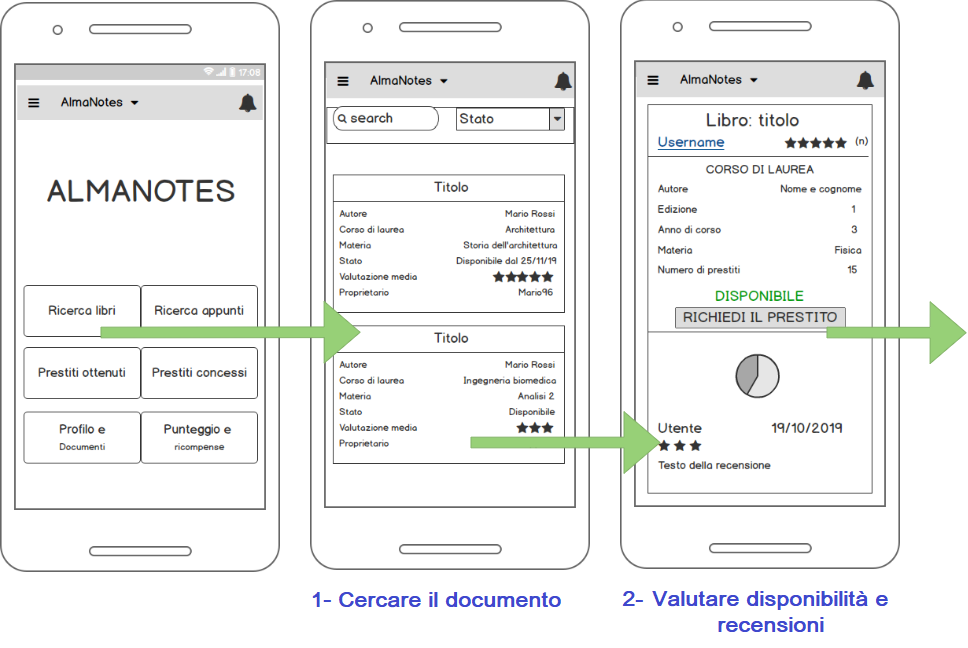
\includegraphics[width=0.95\linewidth]{images/storyboard1.png}
\end{figure}
\end{frame}
\begin{frame}
\frametitle{Storyboard: Prendere in prestito un documento (2)}
\begin{figure}
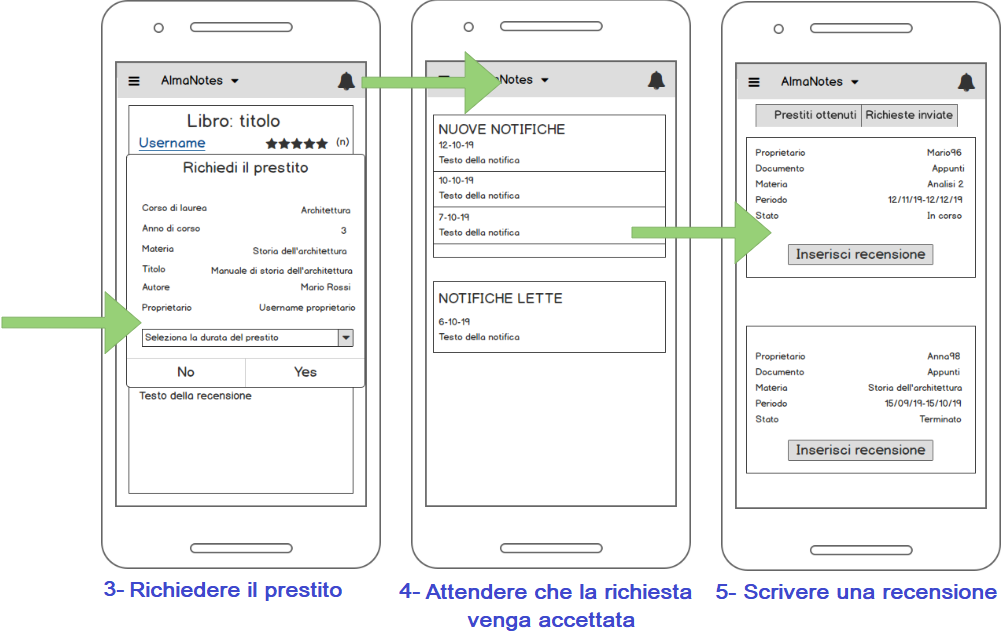
\includegraphics[width=0.95\linewidth]{images/storyboard2.png}
\end{figure}
\end{frame}
\begin{frame}
\frametitle{Storyboard: Cedere in prestito un documento (1)}
\begin{figure}
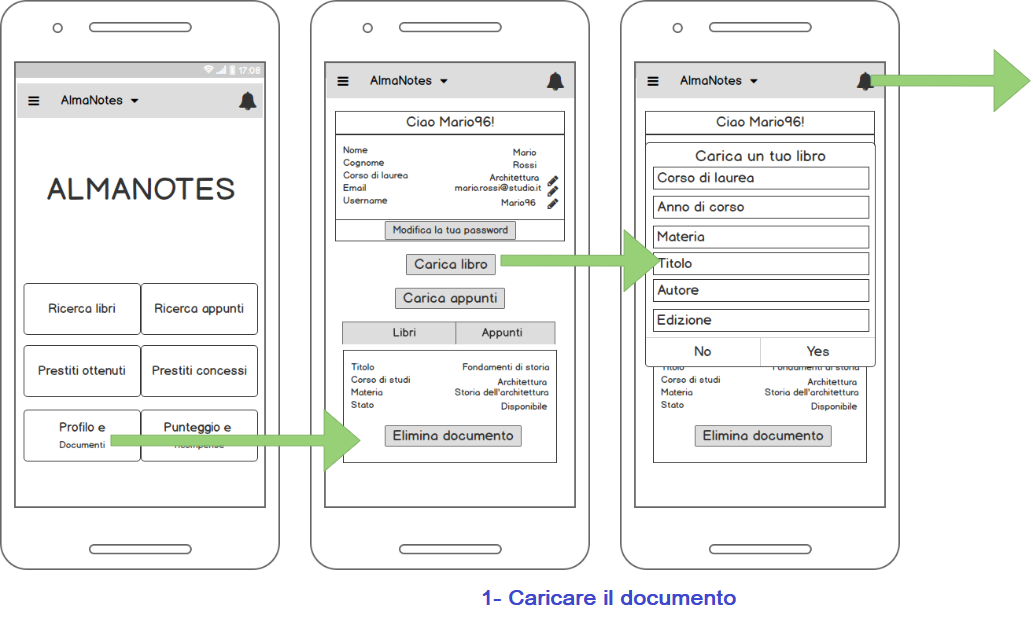
\includegraphics[width=0.95\linewidth]{images/storyboard3.png}
\end{figure}
\end{frame}
\begin{frame}
\frametitle{Storyboard: Cedere in prestito un documento (2)}
\begin{figure}
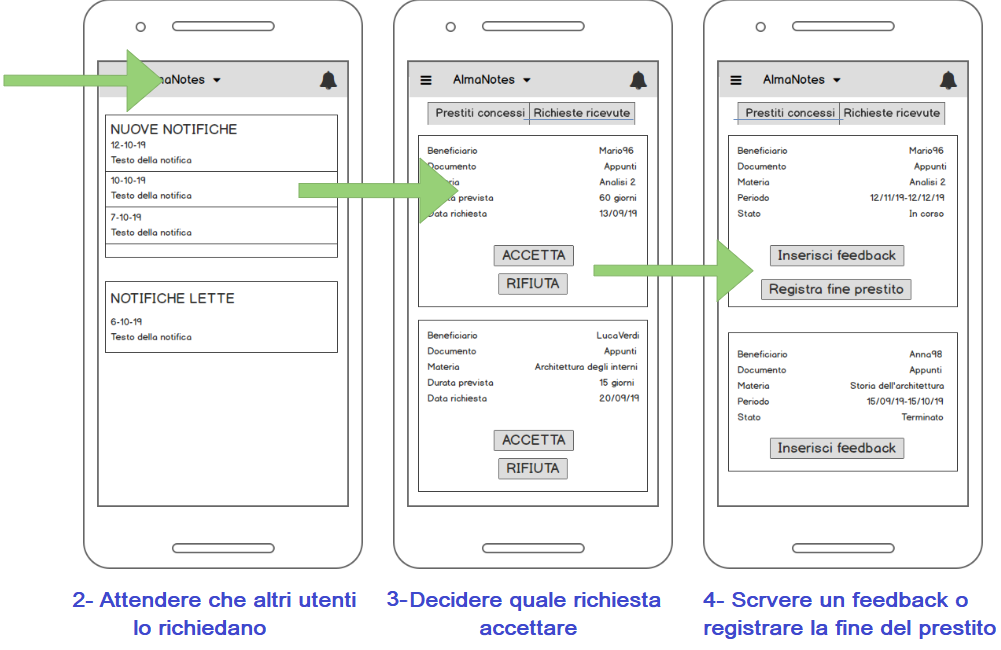
\includegraphics[width=0.95\linewidth]{images/storyboard4.png}
\end{figure}
\end{frame}
\begin{frame}
\frametitle{Storyboard: Ottenere credito valido per l'acqua}
\begin{figure}
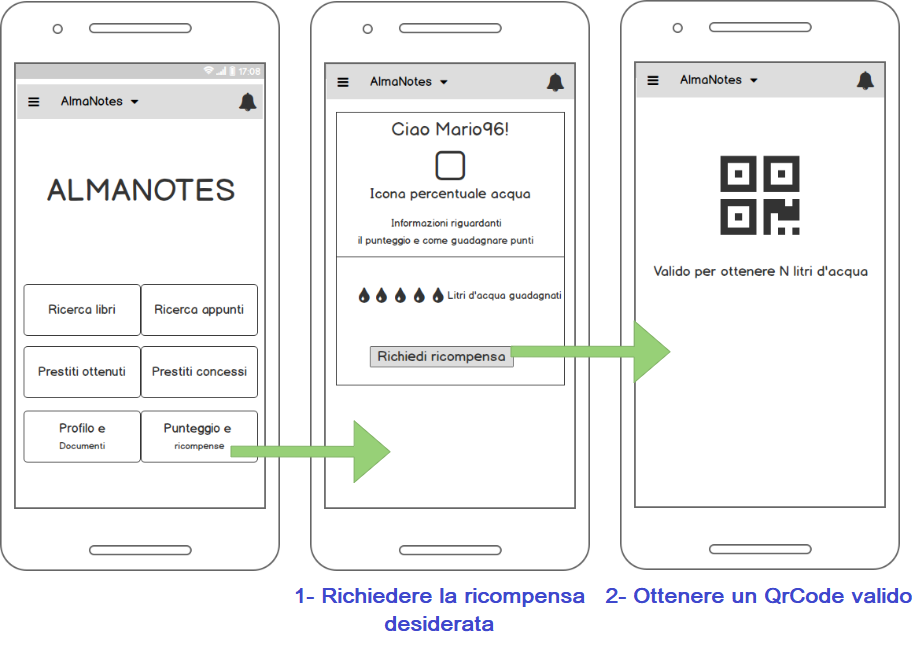
\includegraphics[width=0.90\linewidth]{images/storyboard5.png}
\end{figure}
\end{frame}
%------------------------------------------------
\subsection{Focus Group}

\begin{frame}
\frametitle{Focus Group: Planning}
\begin{itemize}
\item Nel focus group sono state coinvolte 8 persone, scelte tra amici e compagni di corso, in grado di impersonare gli utenti target dell'applicazione.
\item Gli argomenti trattati durante il focus group sono stati i seguenti: 
\begin{itemize}
\item Applicazione web in generale.
\item Cercare e prendere in prestito un documento.
\item Caricare e cedere in prestito un documento.
\item Ottenere credito valido per l'acqua.
\end{itemize}
\item Le storyboard e i mockup navigabili realizzati con Balsamiq sono stati utili per mostrare agli utenti la possibile interazione con il sistema e per raccogliere feedback relativi agli argomenti proposti.
\end{itemize}
\end{frame}
\begin{frame}
\frametitle{Focus Group: Results}
La conduzione del focus group ha evidenziato alcune esigenze degli utenti:
\begin{itemize}
\item Per quanto riguarda la ricerca di libri o appunti, è emersa la necessità di specificare anche più campi di ricerca contemporaneamente.
\item Gli utenti, pur avendo ben compreso il meccanismo di richiesta dei documenti, hanno mostrato alcune difficoltà nella gestione del prestito, che ha inizio non appena una richiesta viene accettata.
\item Un altro feedback raccolto riguarda la possibilità di contattare in modo semplice ed immediato un altro utente (ad esempio, per accordarsi per lo scambio del documento).
\item Alcuni utenti hanno espresso il desiderio di trovare nell'applicazione una sezione contenente informazioni relative alle varie funzionalità disponibili e a come utilizzarle (una sorta di “guida utente”).
\end{itemize}
\end{frame}
%------------------------------------------------

\section{Sviluppo}

%------------------------------------------------
\subsection{Client}

\begin{frame}
\frametitle{Sviluppo Client}
\begin{itemize}
\item Stack MEVN (MongoDB, Express, \textbf{Vue}, Node).
\item \textit{Single Page Application} realizzata con \textit{Vue CLI} e completamente indipendente rispetto al server.
\item Organizzazione in \textit{Componenti}, spesso riutilizzati e che comunicano tra di loro tramite \textit{Props} e \textit{Event Bus}. Creati \textit{Mixin} per condividere codice tra componenti e sfruttato \textit{Vue Router} per la navigazione.
\item Interfaccia grafica realizzata con \textit{Vuetify}, framework per sviluppare applicazioni \textit{Responsive} per Vue. L'interfaccia grafica è \textit{Mobile First} ed è stata seguita la strategia del \textit{Progressive Enhancement}.
\item Utilizzate librerie \textit{D3} e \textit{ChartJS} per \textit{Data Visualization}.
\item \textit{Socket.IO Client} per ricevere real time le notifiche inviate dal server.
\item \textit{Qrcodejs} e \textit{jsPDF} per generare ed esportare dei QrCode. 
\item \textit{Vuelidate} per la validazione dell'input dell'utente nei vari form.
\item \textit{Progressive Web Application} sfruttando il supporto messo a disposizione da Vue CLI: l'applicazione è installabile.
\end{itemize}
\end{frame}
%------------------------------------------------
\subsection{Server}

\begin{frame}
\frametitle{Sviluppo Server}
\begin{itemize}
\item Stack MEVN (\textbf{MongoDB}, \textbf{Express}, Vue, \textbf{Node}).
\item Applicazione \textit{Node} realizzata con \textit{Express} e che espone delle \textit{API RESTful}. Il server è robusto, gestisce l'autenticazione e restituisce opportuni errori se necessario (input errato, utente non autorizzato).
\item Come database è stato usato \textit{MongoDB}, ed è stato sfruttato \textit{Mongoose} per definire schemi (relativi alle varie entità) e query.
\item \textit{MongooseDiscriminators} per ereditarietà tra schemi (es: definito schema ``documento'', da cui ereditano sia ``libro'' sia ``appunti'').
\item Per quanto riguarda la sicurezza, le password degli utenti vengono criptate (nel db sono salvati hash delle password e valori di sale usati). 
\item Usati \textit{Tensorflow.js} e il modello \textit{Toxicity} per riconoscere recensioni e feedback non appropriati (contenenti insulti, minacce e oscenità).
\item Libreria \textit{Socket.IO} per inviare notifiche push ai client.
\item \textit{Nodemailer} per inviare email direttamente dall'applicazione.
\item Deploy online dell'applicazione grazie a \textit{Heroku} (PaaS), sfruttando un database anch'esso su cloud (il SaaS \textit{MongoDB Atlas}).
\end{itemize}
\end{frame}
%------------------------------------------------

\section{Testing}

%------------------------------------------------
\subsection{Nielsen’s Heuristics}

\begin{frame}
\frametitle{Testing: Nielsen’s Heuristics}

Nello sviluppo dell'applicazione, sono stati seguiti i metodi proposti dalle euristiche di Nielsen. Di seguito, sono riportate alcune regole adottate:
\begin{itemize}
\item \textbf{Visibilità dello stato del sistema}: l'applicazione cerca di far capire agli utenti cosa sta accadendo tramite, ad esempio, alert o notifiche.
\item \textbf{Corrispondenza tra il sistema e il mondo reale}: l'applicazione utilizza parole appartenenti al linguaggio naturale e icone comuni.
\item \textbf{Prevenzione degli errori e careful design}: il sistema richiede una conferma prima  dell'esecuzione di ogni operazione non banale.
\item \textbf{Riconoscere anziché ricordare}: gli utenti non devono ricordare le informazioni, ma poterle visualizzare (es: campi ricerca avanzata).
\item \textbf{Aiutare gli utenti a riconoscere e risolvere gli errori}. Un esempio è la validazione dell'input dell'utente, che avviene già durante l'inserimento e non solo nel momento del submit.
\item \textbf{Aiuto e documentazione}: informazioni nella pagina “Scopri di più”.
\end{itemize}
\end{frame}
%------------------------------------------------
\subsection{Usability testing}

\begin{frame}
\frametitle{Testing: Usability testing}
Un'altra tecnica di testing utilizzata in fase di sviluppo è stata l'usability testing: le varie funzionalità dell'applicazione, man mano che venivano implementate, sono state testate da utenti reali per valutare l'usabilità del sistema. Mediante il protocollo Think Aloud, sono state raccolte le considerazioni degli utenti e queste hanno consentito di migliorare l'applicazione. Alcune delle modifiche apportate sono elencate di seguito:
\begin{itemize}
\item Vari cambiamenti/miglioramenti nell'interfaccia grafica.
\item In un primo momento, il sistema richiedeva l'autenticazione per accedere a ogni pagina, ma è risultato essere più usabile se l'avesse richiesta solo quando necessaria (profilo, gestione prestiti).
\item Nell'inserimento di un nuovo documento, inizialmente tutti i campi richiesti dovevano essere inseriti manualmente. In seguito, si è scelto di rendere guidata la scelta in alcuni campi (corso di laurea, materia).
\item Nell'homepage, è stata aggiunta una didascalia che descrive in breve lo scopo dell'applicazione (senza accedere alla pagina “Scopri di più”).
\end{itemize}
\end{frame}
%------------------------------------------------

\section{}

\begin{frame}
\Huge{\centerline{Grazie per l'attenzione!}}
\end{frame}

%------------------------------------------------

\end{document} 